
\documentclass[8pt]{beamer}

\usepackage[english]{babel}
\usepackage[utf8]{inputenc}
\usepackage{pdfpages}
\usepackage{color}
\usepackage{graphicx, import}
\usepackage{amsmath}
\usepackage{amssymb}
\usepackage{amsthm}
\usepackage{tikz}
\usepackage[numbers, square]{natbib}
\usepackage{mathtools}

\usetikzlibrary{external, positioning, fit}
\tikzexternalize[prefix=figures/]


\bibliographystyle{plainnat}
\usetheme{metropolis}
\setbeamertemplate{frame footer}{\insertshortauthor\hfill\insertshortinstitute}
\setbeamercolor{footline}{fg=gray}


\title[]{Weakly Supervised 2D to 3D Lifting of Human Poses}
\author[Nikolas Klug]{Nikolas Klug}
\institute[University of Augsburg]{University of Augsburg}
\date{21 August 2019}


\begin{document}
	\frame{\titlepage}
	
	\begin{frame}[t]{The Problem}
		This work is based on \\
		\vspace{5pt}
		\emph{Can 3D Pose be Learned from 2D Projections Alone?}\linebreak
		\begin{footnotesize}
			Dylan Drover, Rohith MV, Ching-Hang Chen, Amit Agrawal, Ambrish Tyagi, and Cong Phuoc Huynh.\linebreak
			In Computer Vision -- ECCV 2018 Workshops, Pages 78-94, 2019. Springer International Publishing.\par
		\end{footnotesize}
		\vspace{2cm}
		Features:
		\begin{itemize}
			\item Lifting human 2D poses to 3D
			\item Using only 2D poses -- no ground truth required
		\end{itemize}
	\end{frame}

	\begin{frame}{Why?}
		\begin{itemize}
			\item Massive amount of 2D images/videos available
			\item Very good 2D keypoint detectors out there: Stacked Hourglass, OpenPose etc.
			\item Getting 3D ground truth data is hard and expensive
		\end{itemize}
	\end{frame}

	\begin{frame}{How It Works}
		\begin{figure}
	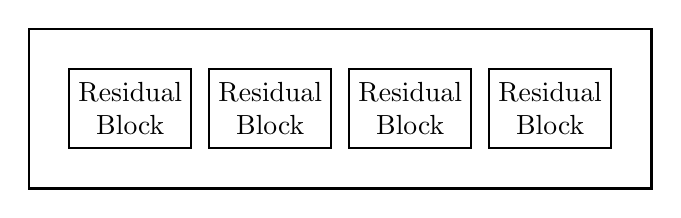
\begin{tikzpicture}
%		\draw (1, 1) rectangle ++(2,1);
%		\draw (4, 1) rectangle ++(2,1);
%		\node (a) at (1, 1) [draw,thick,minimum width=4cm,minimum height=2cm] {};
		\node[] (a1) [draw, thick, minimum width=1cm,minimum height=1cm, align=center] {Residual\\ Block};
		\node[right=.2 of a1] (a2) [draw, thick, minimum width=1cm,minimum height=1cm, align=center] {Residual\\ Block};
		\node[right=.2 of a2] (a3) [draw, thick, minimum width=1cm,minimum height=1cm, align=center] {Residual\\ Block};
		\node[right=.2 of a3] (a4) [draw, thick, minimum width=1cm,minimum height=1cm, align=center] {Residual\\ Block};
		\node[inner sep=.5cm, fit=(a1)(a2)(a3)(a4)] (generator) [draw, thick] {};
		
%		\node[right=1 of a] (b) [draw,thick,minimum width=2cm,minimum height=1cm] {};
%		\path[->] (a) edge [] (b);
	\end{tikzpicture}
	\caption{Figure of the system proposed by }
\end{figure}
	\end{frame}

	\begin{frame}{Results}
		
	\end{frame}
	
	\begin{frame}{My Contribution}
		\begin{itemize}
			\item Introduction of \emph{Limb Loss}
			\item Analysis of the Effects of Normalization
		\end{itemize}
	\end{frame}
	
	
\end{document}